\documentclass{article}



% if you need to pass options to natbib, use, e.g.:
%     \PassOptionsToPackage{numbers, compress}{natbib}
% before loading neurips_2024


% ready for submission
\usepackage{neurips_2024}


% to compile a preprint version, e.g., for submission to arXiv, add add the
% [preprint] option:
%     \usepackage[preprint]{neurips_2024}


% to compile a camera-ready version, add the [final] option, e.g.:
%     \usepackage[final]{neurips_2024}


% to avoid loading the natbib package, add option nonatbib:
%    \usepackage[nonatbib]{neurips_2024}


\usepackage[utf8]{inputenc} % allow utf-8 input
\usepackage[T1]{fontenc}    % use 8-bit T1 fonts
\usepackage{hyperref}       % hyperlinks
\usepackage{url}            % simple URL typesetting
\usepackage{booktabs}       % professional-quality tables
\usepackage{amsfonts}       % blackboard math symbols
\usepackage{nicefrac}       % compact symbols for 1/2, etc.
\usepackage{microtype}      % microtypography
\usepackage{xcolor}         % colors
\usepackage{graphicx}
\usepackage{amsfonts}
\usepackage{amsmath}
\usepackage{amssymb}
\usepackage{amsthm}
\usepackage{subfig}
\usepackage{float}
\usepackage{bbm}
\usepackage{bm}

\theoremstyle{plain}
\newtheorem{theorem}{Theorem}[section]
\newtheorem{proposition}[theorem]{Proposition}
\newtheorem{lemma}[theorem]{Lemma}
\newtheorem{corollary}[theorem]{Corollary}
\theoremstyle{definition}
\newtheorem{definition}[theorem]{Definition}
\newtheorem{assumption}[theorem]{Assumption}
\theoremstyle{remark}
\newtheorem{remark}[theorem]{Remark}

\title{Contrastive Optimization -- Preliminaries}


% The \author macro works with any number of authors. There are two commands
% used to separate the names and addresses of multiple authors: \And and \AND.
%
% Using \And between authors leaves it to LaTeX to determine where to break the
% lines. Using \AND forces a line break at that point. So, if LaTeX puts 3 of 4
% authors names on the first line, and the last on the second line, try using
% \AND instead of \And before the third author name.


\author{%
  David S.~Hippocampus\thanks{Use footnote for providing further information
    about author (webpage, alternative address)---\emph{not} for acknowledging
    funding agencies.} \\
  Department of Computer Science\\
  Cranberry-Lemon University\\
  Pittsburgh, PA 15213 \\
  \texttt{hippo@cs.cranberry-lemon.edu} \\
  % examples of more authors
  % \And
  % Coauthor \\
  % Affiliation \\
  % Address \\
  % \texttt{email} \\
  % \AND
  % Coauthor \\
  % Affiliation \\
  % Address \\
  % \texttt{email} \\
  % \And
  % Coauthor \\
  % Affiliation \\
  % Address \\
  % \texttt{email} \\
  % \And
  % Coauthor \\
  % Affiliation \\
  % Address \\
  % \texttt{email} \\
}


\begin{document}


\maketitle


% \begin{abstract}
%   The abstract paragraph should be indented \nicefrac{1}{2}~inch (3~picas) on
%   both the left- and right-hand margins. Use 10~point type, with a vertical
%   spacing (leading) of 11~points.  The word \textbf{Abstract} must be centered,
%   bold, and in point size 12. Two line spaces precede the abstract. The abstract
%   must be limited to one paragraph.
% \end{abstract}


\section{Background \& Motivation}

The standard optimization pipeline for image classification predominantly consists of using a CNN-backbone with a fully-connected layer pointing to the classification targets.

This setup is vulnerable to spurious correlation caused by features like a common background, causing the model to learn `tricks', bypassing actually learning the target features. A simple example is illustrated in the second paragraph of the introduction in \cite{arjovsky2020invariantriskminimization}.

A popular post-hoc technique -- Class Activation Mappings \citep{zhou2016learning} -- helps diagnose this by generating a heatmap that visualizes the regions of the image used by the model to generate the prediction. Further research uncovered that the interpretation used by CAMs, and it's derivative GradCAMs were unfaithful as a consequence of the averaging step.

HiResCAM \citep{draelos2020use} is a variant of GradCAM \citep{selvaraju2017grad} that demonstrates that their visualization \textbf{provably recovers the input-dependent abnormality score} from the final classification. Therefore, there is a guarantee associated with the faithfulness of the visualization.

This approach derives an interpretable training objective using HiResCAMs, which replaces and outperforms cross-entropy loss to build an intrinsically interpretable, performant model.

\section{Methodology}

The experimental setup is a CNN-backbone (here, ResNet-50) with a single fully connected softmax-activated layer for classification. The backbone outputs feature maps $\bm{A} \in \mathbb{R}^{F \times D_1 \times D_2}$, which is flattened to $\bm{A}_F \in \mathbb{R}^{FD_1D_2 \times 1}$ and fed to the linear layer with $\bm{w}_c \in \mathbb{R}^{1 \times FD_1D_2}$. The logits obtained in $\mathbb{R}^{c}$, where $c$ is the total number of classes is then passed through softmax to generate the final probabilities.

\subsection{Observation: HiResCAMs Explain Class Score, Not Class Probabilites}

Per \cite{draelos2020use}, a HiResCAM is defined as follows:
\begin{gather}
	\tilde{\mathcal{\bm{A}}}_c^{\text{HiResCAM}} = \sum^F_{f=1} \frac{\partial s_c}{\partial \bm{A}^f} \odot \bm{A}^f
\end{gather}

Where $s_c$ denotes the logit for a single class. $\tilde{\mathcal{\bm{A}}}_c^{\text{HiResCAM}}$ generates a class-specific CAM. For the CAM architecture, \cite{draelos2020use} (section 3.6.2) shows that:
\begin{gather}
	\sum^{D_1,D_2}_{i,j} \tilde{\mathcal{\bm{A}}}_{c,i,j}^{\text{HiResCAM}} = \frac{\bm{w}_c \bm{A}_F}{D_1 D_2} \\
	s_c = \frac{\bm{w}_c \bm{A}_F}{D_1 D_2} + b_c = \sum^{D_1,D_2}_{i,j} \tilde{\mathcal{\bm{A}}}_{c,i,j}^{\text{HiResCAM}} + b_c
\end{gather}
Therefore, we can recreate the entire input-dependent part of the score using HiResCAMs. Doing this for each class $c$, we obtain the bias-removed logit vector $\in \mathbb{R}^{c}$.

The standard interpretation of this result uses the obtained activation maps as explanations for the prediction. Popular practice is to follow this up by ReLU and normalization \citep{draelos2020use}. However, since softmax is computed over the logit vector, this interpretation is flawed.

We can consider the backbone as a kernel that attempts to linearly separate the correct class, with the softmax-activated final layer just being logistic regression over the final feature map.

In this setup, each class has it's own set of weights that feedforwards independently, but trains collaboratively. It assigns a score for it's specific value, which is independent since one set of weights does not affect the other over a forward pass. A consequence of performing softmax over the final logits is that the normalization steps renders only the difference between each score $s_c$ relevant for the final prediction probability.

\begin{theorem}\label{classprobdiff}
	Individual class probabilites $\sigma_c(\bm{s})$ depend on the difference(s) between class logits.
\end{theorem}
\begin{proof} Individual class probabilities for logit vector $\bm{s}$ are defined as:
	\begin{gather}
		\sigma_c(\bm{s}) = \frac{e^{s_c}}{\sum_i e^{s_i}}
	\end{gather}
	We define our logit vector in terms of the elementwise difference to a target class $c$:
	\begin{gather}
		d = [s_i - s_c]_i \\
		\bm{s} = [s_c + d_i]_i
	\end{gather}
	Based on this definition, class probabilities can now be computed as:
	\begin{align}
		\sigma_c(\bm{s}) &= \frac{e^{s_c}}{\sum_i e^{s_c+d_i}} \\
				 &= \frac{e^{s_c}}{e^{s_c} \sum_i e^{d_i}} = \frac{1}{\sum_i e^{d_i}}
	\end{align}
	This recontextualizes softmax as a direct function of the differences of class logits.
\end{proof}
\begin{corollary} Since class probabilities depend on logit differences, the class probabilities are identitical for any two pairs of logit vectors with identical logit differences.
	\begin{gather}
		\frac{e^{s_c}}{\sum_i e^{s_i}} = \frac{e^{s_c+r}}{\sum_i e^{s_i+r}} \forall r \in \mathbb{R}
	\end{gather}
\end{corollary}
\begin{proof} Recontextualizing $\bm{s}$ per the previous proposition, we get:
	\begin{align}
		\frac{e^{s_c}}{\sum_i e^{s_c + d_i}} &= \frac{e^{s_c+r}}{\sum_i e^{s_c+d_i+r}} \\
		\frac{e^{s_c}}{e^{s_c}\sum_i e^{d_i}} &= \frac{e^{s_c+r}}{e^{s_c + r} \sum_i e^{d_i}} \\
		\frac{1}{\sum_i e^{d_i}} &= \frac{1}{\sum_i e^{d_i}}
	\end{align}
	Therefore, the absolute scale of a logit does not influence the final class probability.
\end{proof}

As an example, for logits $[1,2]$ and $[-2,-1]$, $\sigma([1,2]) = \sigma([-2,1]) = [0.2689, 0.7311]$. The prediction probabilities remain the same, despite different values for the same score $s_c$. Therefore, making inferences based on \textit{absolute score} results in a misrepresentation of the internal model state. Instead, the objective is to maximize the \textbf{difference between class logits}.

\subsection{Defining the Contrastive Optimization Objective}

We start by \textbf{comparing the contrast} of the activation maps with respect to one another. If for a single point $\bm{A}_{i,j}$, $\bm{w}_c > \bm{w}_{c'}$, that point is more likely to represent the object belonging to class $c$, even if the absolute value of $\bm{w}_{c'}$ is high. This information is lost during the flattening, which embeds positional invariance.

We therefore derive an optimization objective that attempts to maximize the contrast between the two activations maps. For the binary classification case, $(c, c')$ reflects that correct and incorrect class respectively.
\begin{gather}
	\max_{\theta} s_c - s_{c'} \equiv \max_{\theta} \sum^{D_1,D_2}_{i,j} \tilde{\mathcal{\bm{A}}}_{c,i,j}^{\text{HiResCAM}} + b_c - \sum^{D_1,D_2}_{i,j} \tilde{\mathcal{\bm{A}}}_{c',i,j}^{\text{HiResCAM}} - b_{c'}
\end{gather}
Ignoring the bias terms, our new optimization objective is:
\begin{gather}
	\max_{\theta} \sum^{D_1,D_2}_{i,j} \tilde{\mathcal{\bm{A}}}^{\text{contrastive}}_{(c, c'), i, j} ~~\text{ where }~~ \tilde{\mathcal{\bm{A}}}^{\text{contrastive}}_{(c, c')} := \tilde{\mathcal{\bm{A}}}_{c}^{\text{HiResCAM}} - \tilde{\mathcal{\bm{A}}}_{c'}^{\text{HiResCAM}}
\end{gather}
This is equivalent to the original ERM optimization objective, with the difference being the resultant values preserving spatial information in the form of the activation map instead of flattening the feature map. If $\tilde{\mathcal{\bm{A}}}_{c}^{\text{HiResCAM}} - \tilde{\mathcal{\bm{A}}}_{c'}^{\text{HiResCAM}} > 0$, the classification is correct -- if not, the classification is incorrect. 

We can define ContrastiveCAMs as a generalization of the binary case.

\begin{definition}
	Given a set of classes $C$ with $c_t$ being the target class and $c_{t'}$ being a sampled non-target class, we define ContrastiveCAMs as follows:
	\begin{gather}
		\tilde{\mathcal{\bm{A}}}^{\text{contrastive}}_{(c_t, c_{t'})} := \left\{\tilde{\mathcal{\bm{A}}}_{c_t}^{\text{HiResCAM}} - \tilde{\mathcal{\bm{A}}}_{c_{t'}}^{\text{HiResCAM}}\right\}^{|C|-1}_{c_{t'} \in c \setminus c_t}
	\end{gather}
\end{definition}

This enables us to evaluate ContrastiveCAMs in the multiclass setting. This is trivially a generalization of the previous case, as the same formulation applied to a binary classification task returns a set of contrastive maps containing a single element.

To ensure that the model accurately predicts the target class, each contrastive comparison should yield a positive result. Therefore, the multiclass optimization objective under this paradigm is as follows:
\begin{gather}
	\max_{\theta} \sum^{D_1,D_2}_{j,k}\tilde{\mathcal{\bm{A}}}_{(c, c'),j,k}^{\text{contrastive}}\ \forall c' \in \mathbb{Z}_{+}(|C| - 1)
\end{gather}

\subsection{Observation: Cross-Entropy Motivates Learning from Spurious Correlations}

Using contrastive activation maps, we can evaluate the attention maps generated by a \underline{well-trained} model (ImageNet weights, fine-tuned to $99.9\%$ training accuracy, $99.6\%$ validation accuracy) on Oxford-IIIT Pets:

\begin{figure}[h!]
	\centering
	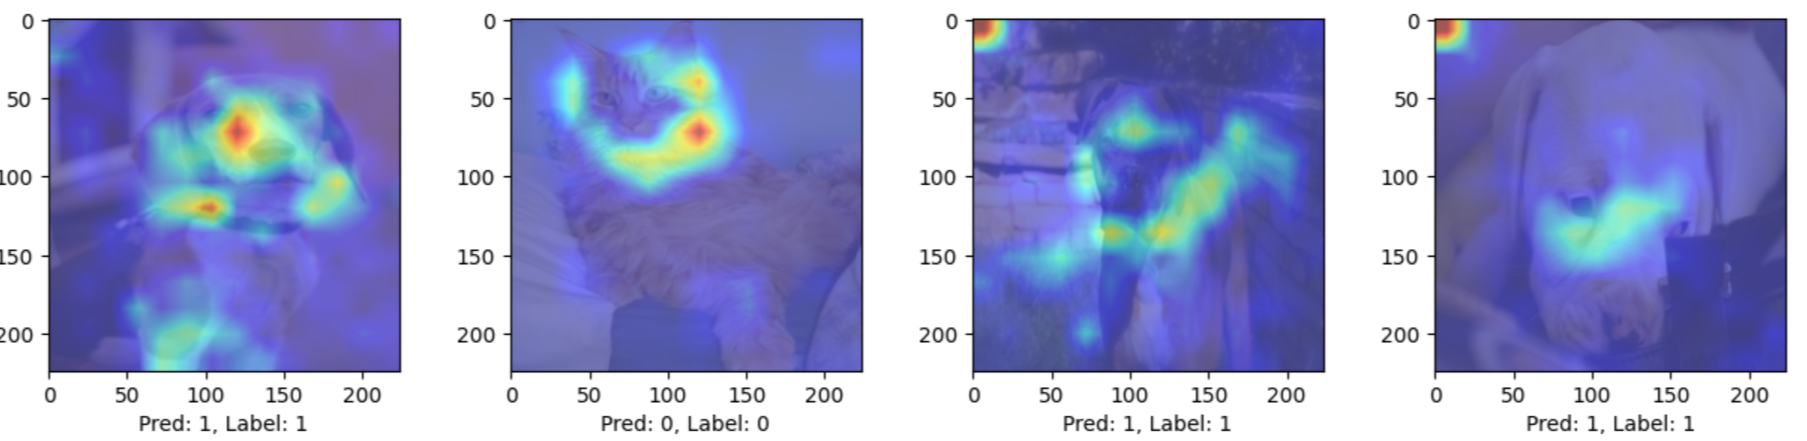
\includegraphics[width=\textwidth]{img/default_cams.png}
\end{figure}

In this random sample, we observe that the regions within each of the images that influence the final prediction are misaligned to the classification target. Particularly, the top-left corner of the final two images contributed significantly to the final prediction, despite not containing the classification target.

Interestingly, this dependence holds even when we average influence plots generated from inference across the dataset:
\begin{figure}[h!]
	\centering
	\subfloat[Pre-Trained on Train]{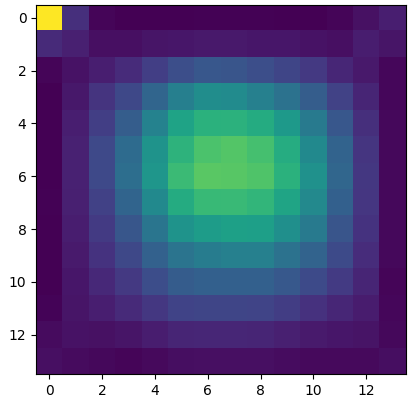
\includegraphics[width=.24\textwidth]{img/default_pretrained_finetuned_best_train_influence.png}}
	\subfloat[Pre-Trained on Valid]{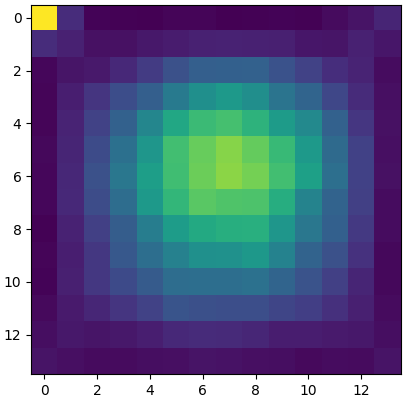
\includegraphics[width=.24\textwidth]{img/default_pretrained_finetuned_best_valid_influence.png}}
	\subfloat[Random Init on Valid]{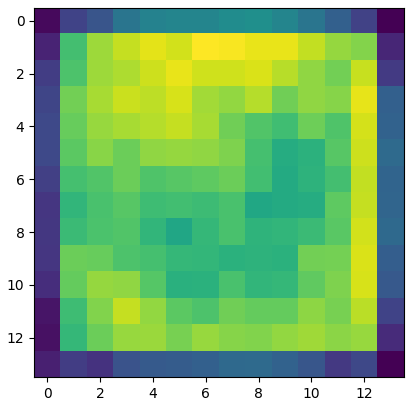
\includegraphics[width=.24\textwidth]{img/default_best_valid_influence.png}}
	\subfloat[Random Init on Train]{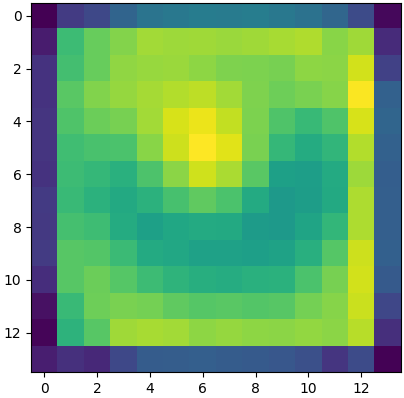
\includegraphics[width=.24\textwidth]{img/default_best_train_influence.png}}
\end{figure}

Further, we can use the segmentation trimaps from the Oxford-IIIT Pets dataset as foreground and background delimiters to bifurcate the regions that influence final prediction logits. On average, we observe the following:

\begin{table}[h]
	\centering
	\begin{tabular}{c|cc|cc}
		\toprule
		\bf Average & \multicolumn{2}{c}{\bf Validation} & \multicolumn{2}{c}{\bf Training} \\
		\bf Pixel Influence & \textbf{Random} & \textbf{Pre-Trained} & \textbf{Random} & \textbf{Pre-Trained} \\
		\midrule
		Foreground & 6.834 & \bf 2.622 & 6.673 & \bf 2.579 \\
		Background & \bf 8.934 & 1.347 & \bf 8.738 & 1.332 \\
		\midrule
		Net & 15.769 & 3.970 & 15.410 & 3.912 \\
		\bottomrule
	\end{tabular}
\end{table}

We observe that weights optimized from random initialization leverage more of the background than the actual target to inform the final prediction. In training classification models, an implicit assumption is that the best approximator of the class label is the target itself, which experimentally are observed to not hold. Despite fine-tuning on pre-trained weights mitigating the problem, it still learnt a feature that can be exploited adversarially.

This is especially concerning for cases wherein the target is far away from the camera, in which case the emphasis is objectively placed on learning the best spurious surrogate to the actual target, rather than obtaining an approximation of the target's feature representation using the fewer available pixels.

% TODO: adversarial ablation

\subsection{Constraining Optimization to an Interpretable Basis}
\label{sec:constraining-optimization}

The primary distinction between the contrastive optimization objective over standard risk is that it preserves spatial information. We know at a pointwise level how each feature contributes to the final prediction.

We can use this to constrain the way optimization occurs -- namely, we only want the model to increase the likelihood of an object belonging to a certain class by actually looking at the features of the class, and not features of spurious correlation like the environment in which the object is present. The model through the process of training should learn to distinguish and subsequently ignore the background in determining the final prediction.

% TODO: formal analysis -- empirical performance test on scale augmentation + norm-change in feature representation.

In addition to learning invariances to spurious correlation, having information about the specific region containing the classification target also motivates learning scale-robust representations of the target. 

\subsubsection{Divergence Minimization}
Segmentation maps describe the region over which the classification target is present. We can leverage this information to define a constrastive cost function as follows:
\begin{gather}
	\{(x, (h, y))\}^N \in \mathcal{D} \text{ where } h_{i,j} := \begin{cases}
		1 & \text{pixel contains subject} \\
		0 & \text{otherwise}
	\end{cases} \\
	D_{KL}(P || Q) := \sum_{i,j} P \cdot \log \frac{P'}{Q} \text{ where } 
	P'_{i,j} := \begin{cases}
		1 & h_{i,j} \neq 0 \\
		P_{i,j} & \text{otherwise}
	\end{cases} \label{d_kl} \\
	\begin{split}
		\mathcal{\bm{J}}(\theta, \mathcal{D}) := &\ \frac{1}{|C|} \sum^{|C|}_{i} \underbrace{\lambda_1 D_{KL}(\sigma_{\text{softmax}}(\lambda_3 h)\ ||\ \sigma_{\text{softmax}}(\lambda_2 \tilde{\mathcal{\bm{A}}}^{\textit{contrastive}}_{(c, i)}))}_{\text{minimize divergence from target shape}} \\
		&+ \underbrace{\frac{\lambda_4}{(|C| - 1) \left(D_1 D_2 - \sum^{D_1,D_2}_{i,j}h_{i,j}\right)} || (1 - h) \odot \tilde{\mathcal{\bm{A}}}^{\textit{contrastive}}_{(c, i)}||^2_F}_{\text{minimize background influence}} \\
		&- \underbrace{\frac{\lambda_5}{(|C| - 1) \sum^{D_1,D_2}_{i,j}h_{i,j}} \sum^{|C|-1,D_1,D_2}_{i,j,k} \left(\tilde{\mathcal{\bm{A}}}^{\textit{contrastive}}_{(c,i)} \odot h\right)_{j,k} }_{\text{maximize foreground influence}}
	\end{split}
\end{gather}

$D_{KL}$ is modified per (10), such that the likelihood comparator sets point probability to 1 if it is part of the foreground. While this violates the probability distribution under which KL Divergence is defined, it motivates the optimizer to maximize the foreground activation, which is especially crucial for cases where the image contains large sections of foreground. During training, observing pointwise divergence revealed that the model was penalized for `over-activating' the foreground, which this modification corrects. In addition, it also averages the divergence from the target segmentation map to each contrastive activation map.

$\lambda_2$ \& $\lambda_3$ are hyperparameters that scale the activation maps, since softmax computed over values with small differences produce largely uniform probability distributions. $\lambda_1$ weighs the importance of the divergence, $\lambda_4$ weights the importance of the background not affecting the final prediction \& $\lambda_5$ weighs the importance of the foreground being positive. For our experiments, $\bm{\lambda} = \{1, 50, 1, 50, 1\}$ were set for $i = \{1, \ldots, 5\}$ respectively. These were identified empirically, without rigorous optimization.

\subsubsection{Ablated Cross-Entropy}

A more mathematically rigorous approach involves performing an ablation over class logits to penalize background influence.

\begin{theorem}\label{ace}
	We can integrate backgroud invariance to the definition of cross-entropy using the following formulation:
	\begin{gather}
		\mathcal{J}(\theta, \mathcal{D}) = -\log \left( \frac{1}{\sum_i \text{exp}\left(-\sum h \odot \tilde{\mathcal{\bm{A}}}^{\text{contrastive}}_{(c, i)} + \sum |(1-h) \odot \tilde{\mathcal{\bm{A}}}^{\text{contrastive}}_{(c, i)}|\right)} \right)
	\end{gather}
\end{theorem}
\begin{proof} Using the definition of HiResCAMs, ContrastiveCAMs and the elementwise difference setup from \ref{classprobdiff}, we have:
	\begin{align}
		d &= [s_i - s_c]_i \\
		&= \left[\sum^{D_1,D_2}_{j,k} \tilde{\mathcal{\bm{A}}}_{i,j,k}^{\text{HiResCAM}} - \sum^{D_1,D_2}_{j,k} \tilde{\mathcal{\bm{A}}}_{c,j,k}^{\text{HiResCAM}}\right]_i \\
		&= \left[ -\sum^{}\tilde{\mathcal{\bm{A}}}^{\text{contrastive}}_{(c, i)} \right]_i
	\end{align}
	As an aside: we note that when $i = c$, the contrastive map obtained is $\bm{0} \in \mathbb{R}^{D_1 \times D_2}$, and instead of $|C| - 1$ contrastive maps we now obtain $|C|$ contrastive maps. \newline \\
	Using our result from \ref{classprobdiff}, we have:
	\begin{gather}
		\sigma_c(\bm{s}) = \frac{1}{\sum_i e^{d_i}} = \frac{1}{\sum_i \text{exp}({-\sum^{}\tilde{\mathcal{\bm{A}}}^{\text{contrastive}}_{(c, i)}})}
	\end{gather}
	For a target class $c$, cross-entropy loss is defined as:
	\begin{gather}
		H(\theta, \mathcal{D}) = -\log \left( \sigma_c(\bm{s}) \right) = -\log \left( \frac{1}{\sum_i \text{exp}({-\sum^{}\tilde{\mathcal{\bm{A}}}^{\text{contrastive}}_{(c, i)}})} \right)
	\end{gather}
	We can break down each contrastive map to foreground and background components:
	\begin{gather}
		H(\theta, \mathcal{D}) = -\log \left( \frac{1}{\sum_i \text{exp}\left({-\sum^{}h \odot \tilde{\mathcal{\bm{A}}}^{\text{contrastive}}_{(c, i)} - \sum (1-h) \odot \tilde{\mathcal{\bm{A}}}^{\text{contrastive}}_{(c, i)}}\right)} \right)
	\end{gather}
	The current loss formulation motivates improving contrast using either the foreground or the background. We penalize contrast on the background, motivating learning invariance to noise in the form of the background.
	\begin{gather}
		\mathcal{J}(\theta, \mathcal{D}) = -\log \left( \frac{1}{\sum_i \text{exp}\left({-\sum^{}h \odot \tilde{\mathcal{\bm{A}}}^{\text{contrastive}}_{(c, i)} + \sum |(1-h) \odot \tilde{\mathcal{\bm{A}}}^{\text{contrastive}}_{(c, i)}}|\right)} \right)
	\end{gather}
	This gives us our ablated cross-entropy formulation.
\end{proof}

In addition to classifying the input image, the model returns a provably accurate attention map used to distinguish between the two classes. This can be obtained by simply computing the absolute values of the contrastive map compared against any two classes, and subsequently performing normalization.

\subsubsection{ACE-Divergence Formulation}

An empirical observation from the behavior of cross-entropy loss is that it displays a tendency to generate contrast only to regions where feature differences are present within the dataset, which places an assumption for the same set of differenciating features being present across the underlying task. In addition, the peaky nature of the generated contrastive maps also encourages vulnerability to adversarial pertubation.

We therefore combined the divergence based loss with ablated cross-entropy. The ablated cross-entropy term ensures accurate predictions using only the region where the classification target is present, and the divergence term mitigates the dataset-specific contrastive setting, motivating effectively learning an implicit segmentation map.

\begin{gather}
	\begin{split}
		\mathcal{\bm{J}}(\theta, \mathcal{D}) := &\ \frac{1}{|C|} \sum^{|C|}_{i} \lambda_1 D_{KL}(\sigma_{\text{softmax}}(\lambda_3 h)\ ||\ \sigma_{\text{softmax}}(\lambda_2 \tilde{\mathcal{\bm{A}}}^{\textit{contrastive}}_{(c, i)})) \\
		&- \lambda_4 \log \left( \frac{1}{\sum_i \text{exp}\left({-\sum^{}h \odot \tilde{\mathcal{\bm{A}}}^{\text{contrastive}}_{(c, i)} + \sum |(1-h) \odot \tilde{\mathcal{\bm{A}}}^{\text{contrastive}}_{(c, i)}}|\right)} \right)
	\end{split}
\end{gather}

For this setting, $\bm{\lambda} = \{1, 50, 1, 10^{-3}\}$ was set for $i = \{1, \ldots, 4\}$ respectively. As in the previous setting, these were identified empirically, without rigorous optimization.

\subsubsection{Ablated Binary Cross-Entropy}

For sigmoid-activated binary / multilabel classification tasks, we leverage similar principles to defined an ablation to binary cross-entropy. Since we do not have a contrastive process in softmax-activation, this definitions relies only on HiResCAMs.

\begin{theorem}\label{abce}
	We can integrate backgroud invariance to the definition of binary cross-entropy using the following formulation:
	\begin{gather}
		H(\theta, \mathcal{D}) = - y_i \log \left(\sigma\left(h \odot \sum_{j,k}\tilde{\mathcal{\bm{A}}}_{i,j,k}^{\text{HiResCAM}} - (1-h) \odot \sum_{j,k}|\tilde{\mathcal{\bm{A}}}_{i,j,k}^{\text{HiResCAM}}|\right) \right) - (1 - y_i) \log \left( \bm{s}_i \right)
	\end{gather}
\end{theorem}
\begin{proof} For any logit $i$, binary cross-entropy loss is defined as:
	\begin{align}
		H(\theta, \mathcal{D}) &= -\left[ y_i \log (\sigma(\bm{s}_i)) + (1 - y_i) \log (1 - \sigma(\bm{s}_i)) \right] \\
		&= -\left[ y_i \log \left(\sigma\left(\sum_{j,k}\tilde{\mathcal{\bm{A}}}_{i,j,k}^{\text{HiResCAM}}\right) \right) + (1 - y_i) \log \left(1 - \sigma\left(\sum_{j,k}\tilde{\mathcal{\bm{A}}}_{i,j,k}^{\text{HiResCAM}}\right) \right) \right]
	\end{align}
	Similar to Theorem \ref{ace}, we can break down each HiResCAM to foreground and background components. For a non-target HiResCAM, anything that is not the target is inherently the background. Therefore, it's definition is retrained.
	\begin{gather}
		H(\theta, \mathcal{D}) = - y_i \log \left(\sigma\left(h \odot \sum_{j,k}\tilde{\mathcal{\bm{A}}}_{i,j,k}^{\text{HiResCAM}} - (1-h) \odot \sum_{j,k}\tilde{\mathcal{\bm{A}}}_{i,j,k}^{\text{HiResCAM}}\right) \right) - (1 - y_i) \log \left( \bm{s}_i \right)
	\end{gather}
	The current formulation motivates activating either the foreground or the background for positive classification, and motivates de-activating every pixel of the non-positive class. We penalize activation on the background for the positive class only:
	\begin{gather}
		H(\theta, \mathcal{D}) = - y_i \log \left(\sigma\left(h \odot \sum_{j,k}\tilde{\mathcal{\bm{A}}}_{i,j,k}^{\text{HiResCAM}} - (1-h) \odot \sum_{j,k}|\tilde{\mathcal{\bm{A}}}_{i,j,k}^{\text{HiResCAM}}|\right) \right) - (1 - y_i) \log \left( \bm{s}_i \right)
	\end{gather}
	This gives us the ablated binary cross-entropy formulation.
\end{proof}

\subsection{Training Detail}

% \begin{figure}
% 	\centering
% 	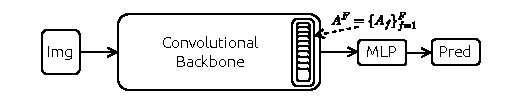
\includegraphics[width=\textwidth]{img/cams.pdf}
% \end{figure}

The Oxford-IIIT Pets dataset is an image dataset with a classification objective alongside high-quality segmentation maps. We train the model on the binary classification case (image containing a dog or cat) as well as the fine-grained, breed specific 37 class split. The architecture used for training was ResNet-50, initialized either with random parameters or ImageNet, with three key modifications:

\paragraph{Removed final downsampling} The final downsampling layer converts the latent feature maps from $D_1 = D_2 = 14$ to $7$. This prohibitively reduces the size of the activation map, and makes it hard to capture relevant features. Therefore, we replace the stride of the final downsampling convolution to $(1,1)$, matching that of the definition used through the rest of ResNet. 

\paragraph{Removed final bias} The linear layer's bias is not used in the computation of the class activation map, and therefore cannot be optimized by the training procedure, as $\nabla_b \mathcal{\bm{J}}(\theta, \mathcal{D})$ = 0. We omit the bias from the final model architecture.

\paragraph{Removed final BatchNormalization \& ReLU} Since the HiResCAM definition for CAM architectures assumes the convolution followed by global average pooling and the final linear layer only, the current explanation does not directly explain the class score. We therefore also neutralize the final two-layers, which successfully recovers the faithfulness guarantee.

\paragraph{Reproducibility.} The source code, dataset, experiments, evals, and model weights can be found at \url{https://dagshub.com/jinensetpal/contrastive-optimization}.

\section{Results}

\subsection{Benchmark: Binary Classification}

For binary classification, the model was trained for $100$ epochs with the Adam optimizer with a learning rate of $10^{-3}$, a batch size of $80$ on a 32GB V100 on a randomly shuffled dataset using the original data splits. The total time for training was $\approx$4hr.

An encouraging result from this experiment is that the model trained on the contrastive objective outperforms the exact same model architecture (with the final bias, batchnorm and ReLU re-added in) on cross entropy loss, even though the control case was trained explicitly to reduce cross entropy.

Our approach's performance on the Oxford-IIIT Pets Dataset to the default is as follows:

\begin{table}[h]
	\centering
	\begin{tabular}{c|ccc}
		\toprule
		\textbf{Method}  & \textbf{Training CE Loss}  & \textbf{Training Accuracy}   & \textbf{Validation Accuracy} \\
		\midrule
		Cross-Entropy & 0.361 & 95.0\% & 82.8\% \\
		Ablated CE (Ours) & 0.333 & 98.4\% & 88.2\% \\
		Ablated CE + KLD (Ours) & \bf 0.322 & \bf 99.2\% & \bf 91.5\% \\
		\bottomrule
	\end{tabular}
\end{table}

This dataset contains a class imbalance (4978 dogs to 2371 cats), however no training modification was made to correct the class imbalance.

\begin{figure}[H]
	\centering
	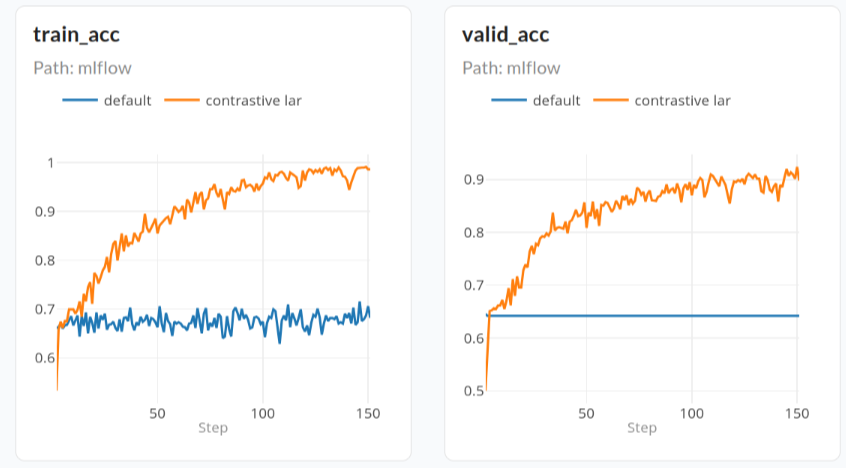
\includegraphics[width=.4\textwidth]{img/accuracy.png}
	\hspace{4em}
	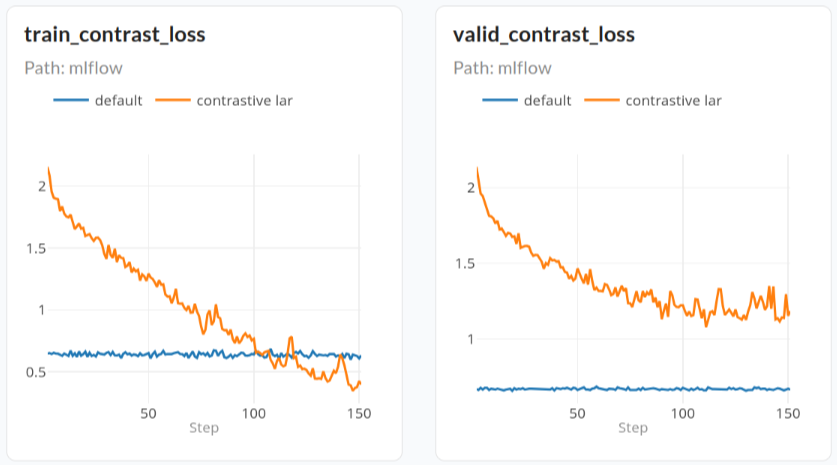
\includegraphics[width=.4\textwidth]{img/loss.png}
	\caption{Plots comparing benchmark cross-entropy loss, training and validation accuracy. The web version of this comparison can be found \href{https://dagshub.com/jinensetpal/contrastive-optimization/experiments\#/compare?experiments=[\%22m_cea5cf4fcbbb4c3f984b2396927cf80c\%22,\%22m_101287828f604122a092a2501ec3facb\%22]}{here}. The orange line represents cross-entropy loss, while the blue line represents the contrastive approach.}
\end{figure}

On comparing contrastive activation maps, we observe in each of the random samples, that the model uses the target region for prediction and not spurious features. In the case of the standard training procedure, this is not the case, and the model does not focus on the target in making it's prediction.

\begin{figure}[H]
	\centering
	\subfloat[Cross-Entropy (CE)]{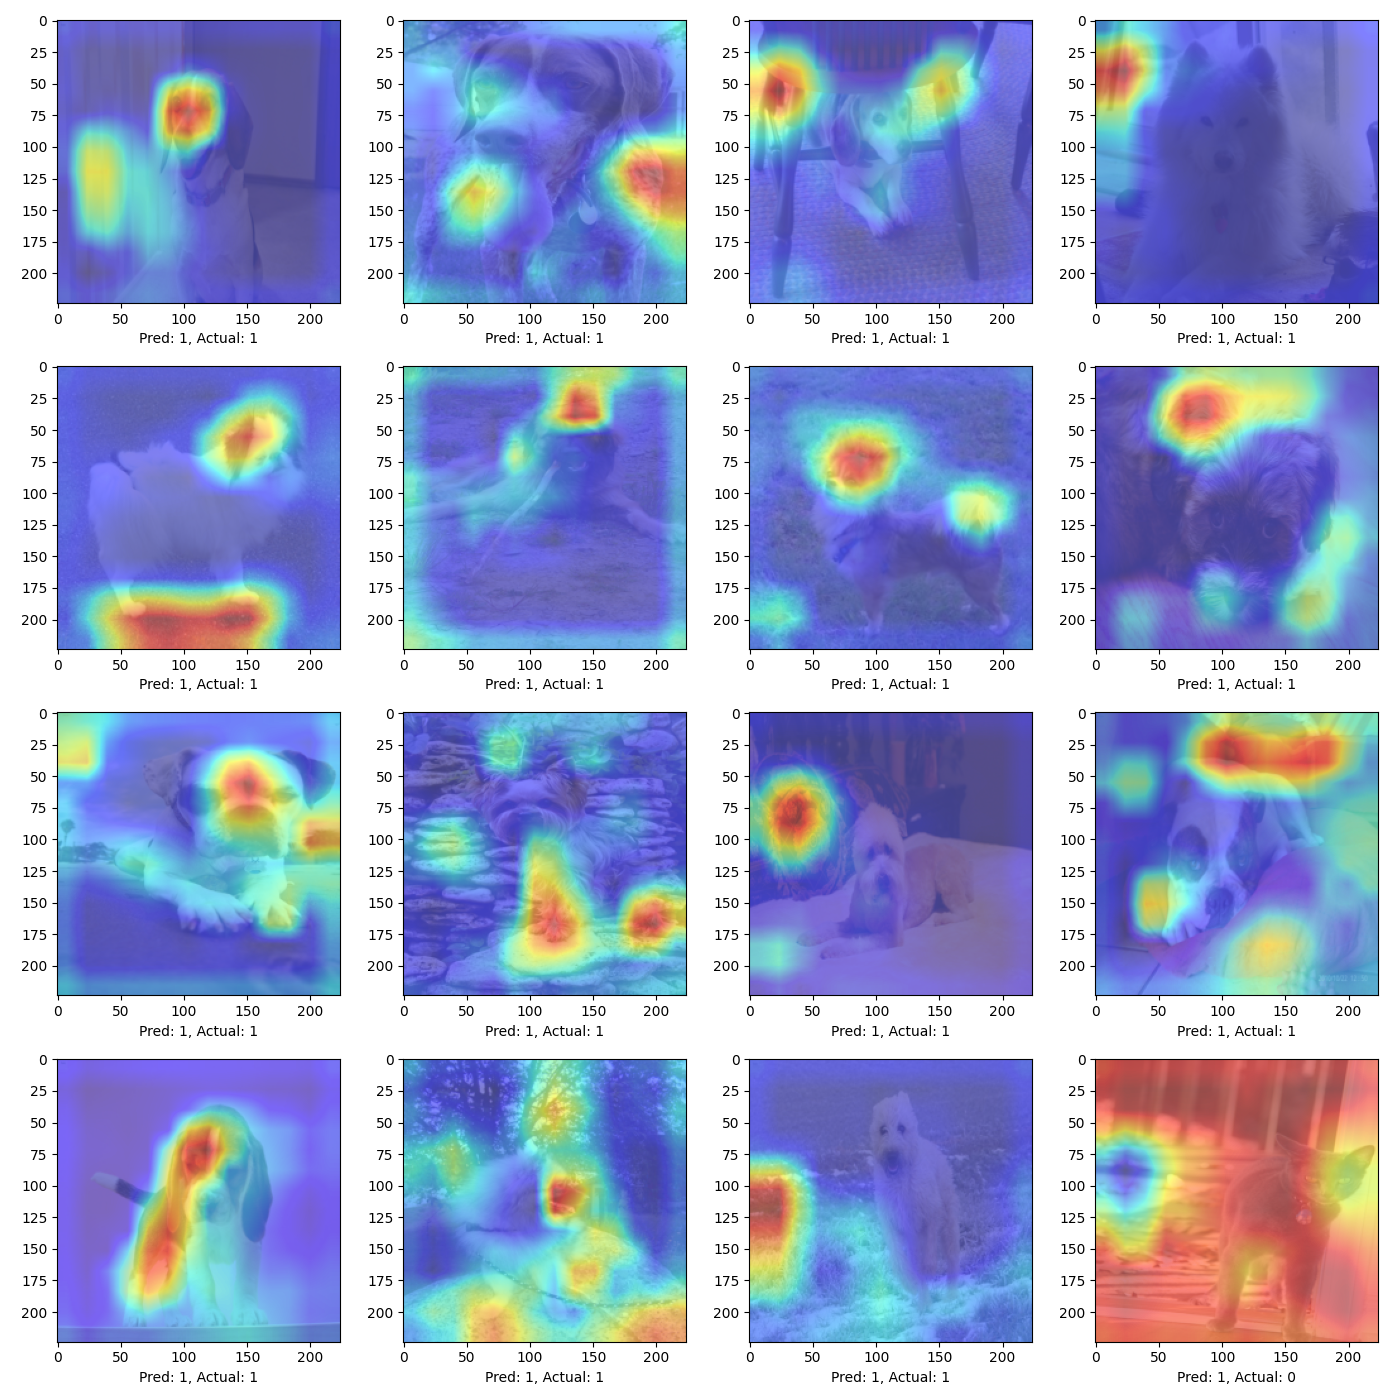
\includegraphics[width=.3\textwidth]{img/default_cam.png}}
	\hspace{1em}
	\subfloat[Ablated CE]{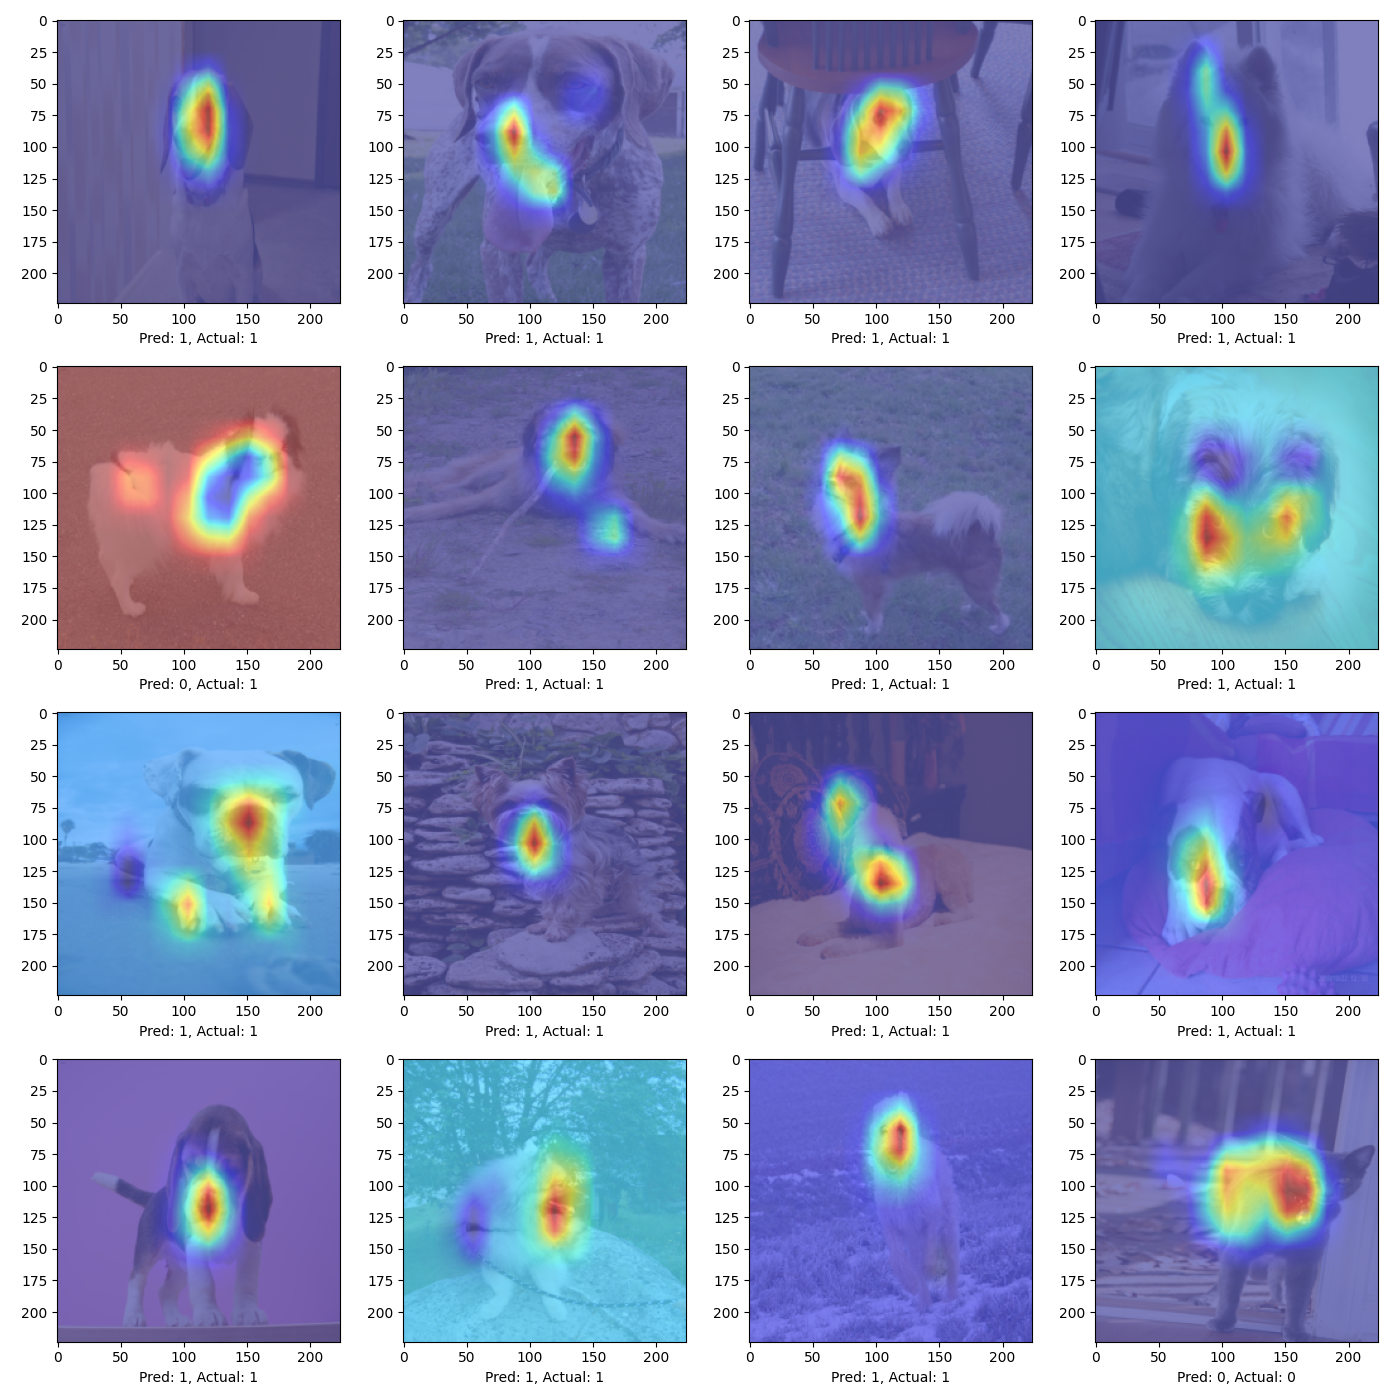
\includegraphics[width=.3\textwidth]{img/contrastive_ace_cam.png}}
	\hspace{1em}
	\subfloat[Ablated CE+KLD]{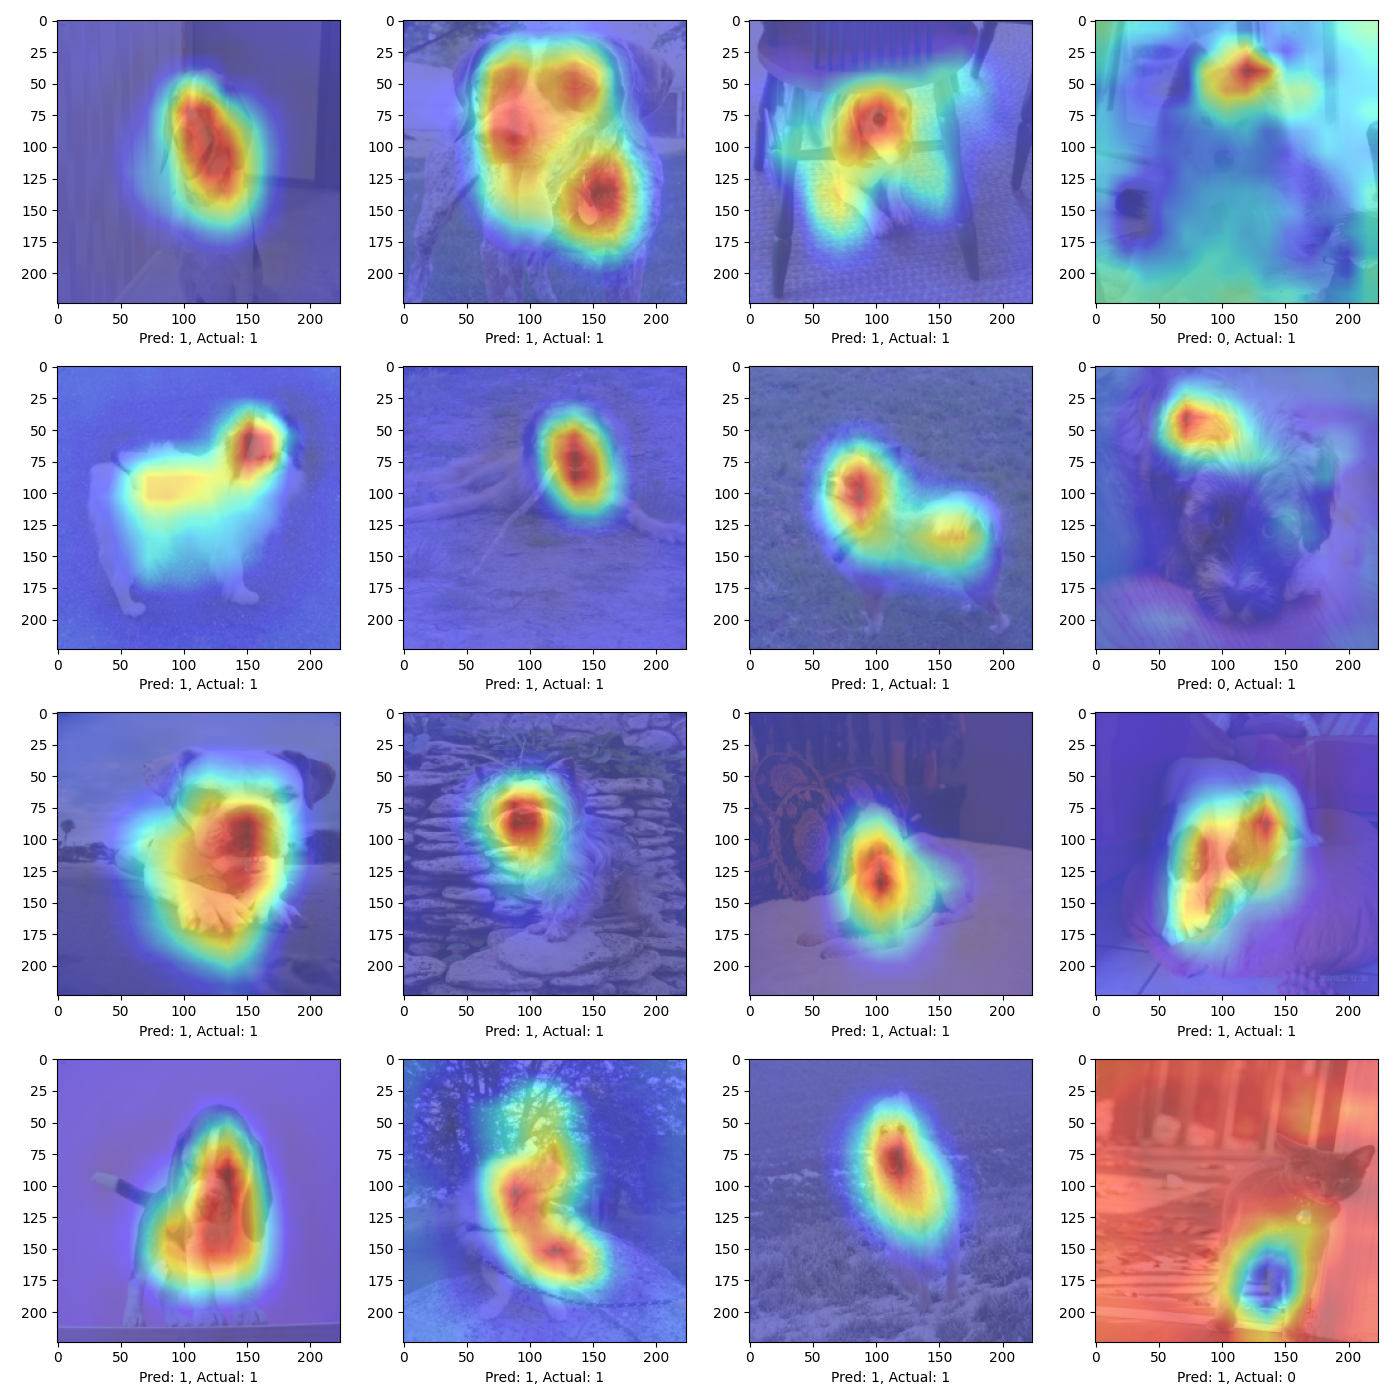
\includegraphics[width=.3\textwidth]{img/contrastive_cam.png}}
	\caption{Contrastive Class Activation Maps from each training setting.}
\end{figure}


\subsection{Benchmark: Multiclass Classification}

For multiclass classification, the objective is to distinguish between the features of species within the cat and dog families. There are a total of 37 classes, with a success of rate of $\approx 2.7\%$ with random guessing. There is virtually no class imbalance in this case.

Our approach's performance on the Oxford-IIIT Pets Dataset to the default is as follows:

\begin{table}[h]
	\centering
	\begin{tabular}{c|ccc}
		\toprule
		\textbf{Method}  & \textbf{Cross Entropy Loss}  & \textbf{Training Accuracy}   & \textbf{Validation Accuracy} \\
		\midrule
		Cross-Entropy & 3.605 & 3.7\% & 5.2\% \\
		Ablated CE (Ours) & 3.610 & 3.1\% & 4.9\% \\
		Ablated CE + KLD (Ours) & \bf 2.743 & \bf 93.0\% & \bf 51.5\% \\
		\bottomrule
	\end{tabular}
\end{table}

We can observe that the default model is unable to learn any valuable information, the contrastive model is able to learn a significant portion of the information, although with a substantial generalization gap.

The contrastive model was trained for 227 epochs with the Adam optimizer with a learning rate of $10^{-3}$ with a batch size of 20, with 4 gradient accumulation steps (effective batch size of 80) on a 32GB V100 on a randomly shuffled dataset using the original splits. The default model was only trained for 33 epochs, while the ablated cross-entropy loss was only trained for 98 epochs by which point both had converged. For posterity, we will run each setup for 227 epochs as well before publication.

\subsection{Benchmark: Out-of-Distribution Generalization}

To test how well the approach generalizes out of the training distribution, we evaluate the performance of the binary classification contrastive model on random samples ($n=1000$) from the \href{https://www.microsoft.com/en-us/download/details.aspx?id=54765}{Kaggle Cats and Dogs Dataset}:
\begin{table}[h]
	\centering
	\begin{tabular}{c|c}
		\toprule
		\textbf{Method} & \textbf{Accuracy} \\
		\midrule
		Cross-Entropy & 77.0\% \\
		Ablated CE (Ours) & 75.7\% \\
		Ablated CE + KLD (Ours) & \bf 83.4\% \\
		\bottomrule
	\end{tabular}
\end{table}

The next goal is to further understand and minimize this generalization gap.

\section{Upcoming / In Progress Tasks} 

\paragraph{Scaling the Approach} Training ResNet-50 on ImageNet and PASCAL VOC can allow us to evaluate if the approach scales effectively, with the performance gain not being constrained to the Oxford-IIIT Pets Dataset.

\paragraph{Understanding the Generalization Gap} While the model for the multiclass paradigm is able to fit the training dataset excellently -- achieving $\approx 93\%$ training accuracy -- the validation accuracy is significantly behind at $\approx 51\%$. This could imply memorization of samples, which was something that this approach was intended to mitigate. Further investigation could help support or disprove this hypothesis.

\paragraph{Evaluating Adversarial Robustness} Could the model looking only at the object to affect the classification score improve adversarial performance?

\paragraph{Mechanistic Interpretability Study} Does the better focus of the model encourage the creation of new image circuits? How does the model perform in cases when it contains neither cat nor dog? Can we make claims about the confidence of the model?

\paragraph{Non-Reduction of Feature Maps} One step of computing HiResCAMs involves summing each attention map to create a single activation map. Could the multiple foci be useful, and something we can further optimize?

\bibliographystyle{plain}
\bibliography{references}

\appendix

\section{Ablated Cross-Entropy Adaptations}

In addition to cross-entropy, we also adapted training methodologies from \citet{imagenetrecipe}. These required additional modifications to the approach. These modifications are discussed in the following sections, remaining consistent with principles discussed in Section \ref{sec:constraining-optimization}.

\subsection{Contrastive CutMix}

CutMix\cite{yun2019cutmix} is a batch-wise augmentation technique that encourages better regularization by a) ``cutting'' out a randomized rectangle (randomized portion remaining consistent across the batch) of a given image and b) ``mixing'' the cut-out with it's neighbor. The corresponding labels are mixed by a randomly sampled parameter $\lambda$. For our experiments, $\lambda \sim \text{Uniform}(0,1)$.

\begin{figure}[h!]
	\centering
	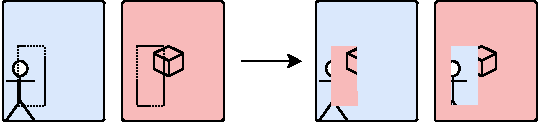
\includegraphics[width=\textwidth]{img/cutmix}
\end{figure}

CutMix can be effectively adapted to work with our setup: given a cut-out, we motivate differential contrast; if non-target pixels are contained in the new image, irresepective of the label, contrast should be generated in favor of the non-target class for the non-target, foreground subset of pixels. This affects the downstream prediction confidence, representative of the label being shifted from one-hot encoding to a randomized affine combination.

Let segmentation mask $h$ take the following form:
\begin{gather*}
	h := \begin{cases}
		-1 & \text{pixel does not contain any class} \\
		c & \text{pixel contains class } c
	\end{cases}
\end{gather*}

Then, Ablated Cross Entropy (\ref{ace}) is formulated as follows:
\begin{gather}
	\mathcal{J}(\theta, \mathcal{D}) = -\log \left( \frac{1}{\sum_i \text{exp}\left(-\sum \mathbbm{1}_{c}(h) \odot \tilde{\mathcal{\bm{A}}}^{\text{contrastive}}_{(c, i)} + \sum |\mathbbm{1}_{-1}(h) \odot \tilde{\mathcal{\bm{A}}}^{\text{contrastive}}_{(c, i)}| + \sum \mathbbm{1}_{i}(h) \odot \tilde{\mathcal{\bm{A}}}^{\text{contrastive}}_{(c, i)} \right)} \right)
\end{gather}

Where the third newly introduced term within the exponent expresses differential contrast.

\end{document}
